\section{Regularization}

\subsection{Data Augmentation}
One way, especially for small datasets as in this case, to reduce overfitting is to use data augmentation, enabling the model to learn from 'more' data. We choose to augment the data in a few different ways since we want to generalize the data so the important features remain. Using augmentation ensures that it will get better accuracy when faced with new images. In other words, it reduces overfitting. By using one image we tested different techniques and found those which fits to this task, see Appendix B - 0.7 Data Augmentation.

The images are of varying quality and taken in different lighting, and this is also what we can expect from the final test set. For this reason we change the brightness, saturation, and contrast. Furthermore, the images are taken from different angles so we rotate the pictures slightly and flip them horizontally. Generally, images of animals are not vertically flipped, so we chose not to do this, but of course, some cases may exist. Also, the images are cropped differently to get finer details from the images, as well as the images becomes scale invariant. Moreover, we shear and translate the images to emulate images taken from different angles of the animal. Even though some of the images are more blurry than others, we chose not to blur the images, as it effectively just reduces the data of the image without reducing input to the model.

The final techniques used as well as augmented sample images using these techniques are shown in Figure \ref{fig:augmentation}.
\begin{figure}[H]
    \vspace*{-0.7cm}
    \centering
    \subfloat[Data Augmentation Techniques.\label{tab:augmentation}]{
        \raisebox{\height}{ % align at the bottom
        \begin{tabular}{|l|p{2.8cm}|}
            \hline
            \textbf{Data Augmentation} & \textbf{Parameters} \\ \hline
            RandomHorizontalFlip & 50\% \\ \hline
            ColorJitter & brightness=0.2 \newline contrast=0.2 \newline saturation=0.2 \newline hue=0 \\ \hline
            RandomAffine & degrees=25 \newline translate=(0.1, 0.1) \newline scale=(0.7, 1.3) \newline shear=(-10, 10) \\ \hline
        \end{tabular}}}
    \hspace{0.4cm}
    \subfloat[Sample images after augmentation.\label{fig:augmentation_images}]{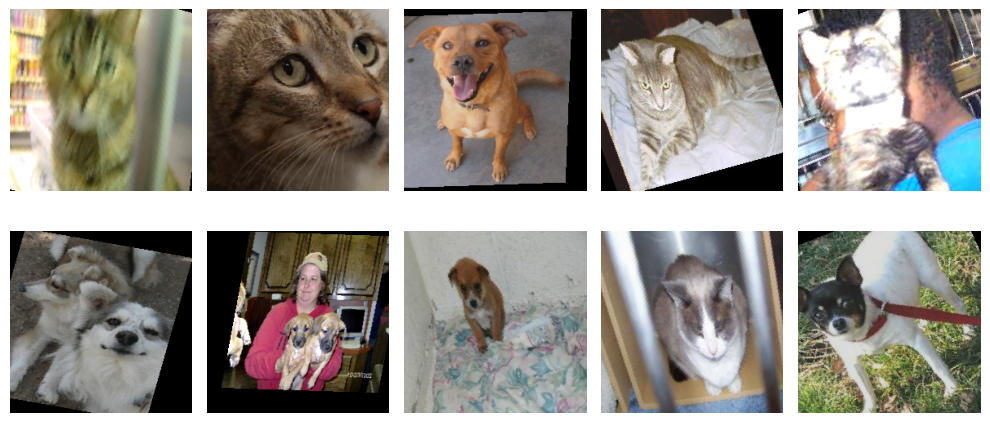
\includegraphics[width=0.5\textwidth]{figures/augmentation.png}}
    \caption{Data augmentation techniques.}
    \label{fig:augmentation}
    \vspace*{-0.7cm}
\end{figure}

The following Figure \ref{fig:augmentation_results} shows the results of running the base model with data augmentation.
\begin{figure}[H]
    \vspace*{-0.7cm}
    \centering
    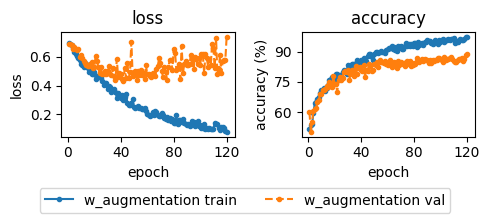
\includegraphics[width=0.4\textwidth]{figures/results_augmentation.png}
    \caption{Results using augmentation.}
    \label{fig:augmentation_results}
    \vspace*{-0.7cm}
\end{figure}
Clearly, the model performs better than without data augmentation and we are now able to train the model for more epochs without overfitting. The training accuracy of the model was $97\%$ with validation accuracy of $88\%$, which indicates that improvements still can be made.

\subsection{More Regularization Techniques}
To achieve even better results, more regularization than just data augmentation is needed. Therefore, we change the base model a bit.

First of all, batch normalization was added to each convolutional layer for stabilizing training and improve convergence. Also, dropout is added to make the model more robust, so no single neurons predicts them all. The results using this model, called 'reg\_1', is shown in Figure \ref{fig:reg1}.

We also experimented with adding weight decay (L2 regularization) to penalize large weights and encourage better generalization. Since it is recommended to use the AdamW optimizer for effective integration of weight decay, we opted for AdamW in this configuration. Also, we halve the learning rate every 25 epochs using 'StepLR'. The results using this model, called 'reg\_2', is shown in Figure \ref{fig:reg1}.
\begin{figure}[H]
    \vspace*{-0.7cm}
    \centering
    \subfloat[Regularized model 1.\label{fig:reg1}]{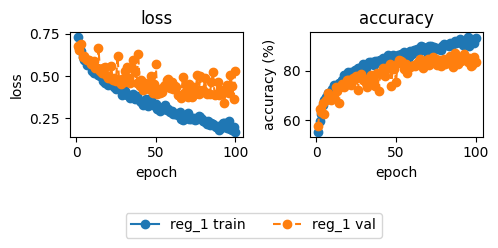
\includegraphics[width=0.4\textwidth]{figures/results_reg_1.png}}
    \hspace{1cm}
    \subfloat[Regularized model 2.\label{fig:reg2}]{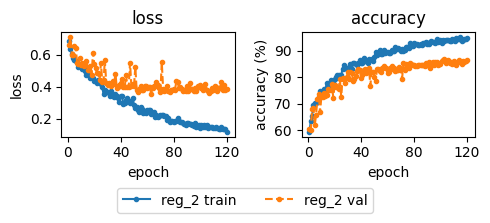
\includegraphics[width=0.4\textwidth]{figures/results_reg_2.png}}
    \caption{Results using regularization.}
    \label{fig:reg}
    \vspace*{-0.7cm}
\end{figure}

From the results, the end accuracy is very similar, however, as expected adding weight decay stabilize the training. The training accuracy of model 'reg\_2' was $93\%$ with validation accuracy of $85\%$. The training- and validation accuracy are now closer to each other, however, no real improvements in terms of validation accuracy is achieved compared to our base model with augmentation.

\subsection{Adding one more convolutional layer}
We wanted to try and improve the model even further, so we increased the number of kernels/features and added an extra convolutional layer, see Table \ref{tab:reg_model}. As before, we ran this model with and without weight decay. The results are shown in Figure \ref{fig:reg}.
\begin{table}[H]
    \vspace*{-0.5cm}
    \centering
    \begin{tabular}{|l|c|c|c|c|c|c|}
    \hline
                & \textbf{Output}                   & \textbf{Kernel}   & \textbf{BatchNorm}    & \textbf{MaxPooling}   & \textbf{Dropout}  & \textbf{Activation}   \\
                & \textbf{kernels/features}         &                   &                       &                       &                   &                       \\ \hline
    Conv2D w/   & 64                                & 3x3               & 64                    & 2x2                   & -                 & ReLU                  \\ \hline
    Conv2D w/   & 128                               & 3x3               & 128                   & 2x2                   & -                 & ReLU                  \\ \hline
    Conv2D w/   & 256                               & 3x3               & 256                   & 2x2                   & -                 & ReLU                  \\ \hline
    Conv2D w/   & 512                               & 3x3               & 512                   & 2x2                   & -                 & ReLU                  \\ \hline
    Conv2D w/   & 512                               & 3x3               & 512                   & 2x2                   & -                 & ReLU                  \\ \hline
    Linear w/   & 512                               & -                 & 512                   & -                     & 40\%              & ReLU                  \\ \hline
    Linear w/   & 256                               & -                 & 128                   & -                     & 20\%              & ReLU                  \\ \hline
    Linear w/   & 2                                 & -                 & -                     & -                     & -                 & -                     \\ \hline
    \end{tabular}
    \caption{Reg4 Model.}
    \label{tab:reg_model}
    \vspace*{-0.8cm}
\end{table}

\begin{figure}[H]
    \vspace*{-0.7cm}
    \centering
    \subfloat[Regularized model 3.\label{fig:reg1}]{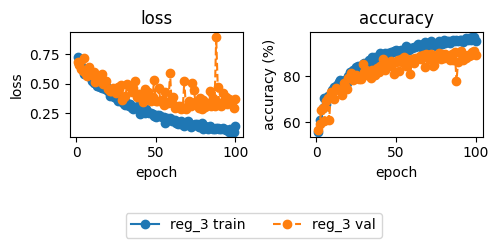
\includegraphics[width=0.4\textwidth]{figures/results_reg_3.png}}
    \hspace{1cm}
    \subfloat[Regularized model 4.\label{fig:reg2}]{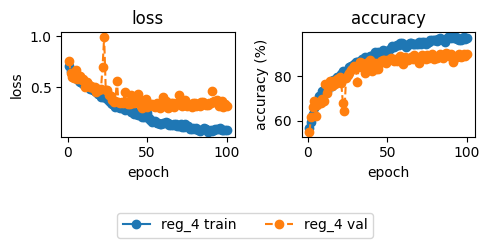
\includegraphics[width=0.4\textwidth]{figures/results_reg_4.png}}
    \caption{Results using one more convolutional layer.}
    \label{fig:reg}
    \vspace*{-0.7cm}
\end{figure}

The training accuracy of model 'reg\_4' was $99\%$ with validation accuracy of $89\%$, indicating some overfitting on the training data. However, we chose to use this model as our final model, as it has the highest validation accuracy.

Based on the feature maps for a sample image of a cat, see Appendix B - 0.10 Predict, we can see that the first layer is mainly edge detection and colors. For the second layer, a lot of the feature maps captures the fur. In the third layer, the faces stands out from the rest of the picture. In the fourth layer there is focus on the head, the ears, and the whiskers.